% !TeX spellcheck = en_GB
\documentclass[../transmission.tex]{subfiles}
\begin{document}
	\section{The lossless transmission line}
		\subsection{Parameters of the lossless line}
			For a \textbf{lossless transmission line}, we say $R' = G' = 0$ in figure \ref{fig:trans_line_lumped_model}. This leads to the following simplifications:
			\begin{itemize}
				\item The \textbf{complex propagation constant} becomes $\gamma = j\omega\sqrt{L'C'}$, meaning that $\alpha$ (the attenuation constant) is 0 and $\beta$ (the phase constant) is $\omega\sqrt{L'C'}$.
				\item The \textbf{characteristic impedance} becomes $Z_0 = \sqrt{\frac{L'}{C'}}=R_0$, a real-valued parameter.
			\end{itemize}
			Here, $L'$ is dependent on $\mu_r$, which is the relative permeability of the dielectric between the two transmission line conductors. $C'$ is dependent on $\epsilon_r$ which is the relative permittivity of the dielectric between the conductors.
			\subsubsection{Characteristic impedance $R_0$}
				The characteristic impedance depends on the geometry of the conductors. We can find three relations which will (without proof) hold true for a lossless transmission line:
				\begin{itemize}
					\item $\sqrt{\frac{\mu_0}{\epsilon_0}}=120\pi$
					\item $R_0\sim \frac{1}{\sqrt{\epsilon_r}}$
					\item $\mu_0\epsilon_0=\frac{1}{c^2}$
				\end{itemize}
				Using these relations, and the assumption that $\mu_r\approx1$ we get:
				\begin{equation}
					\beta = \omega\sqrt{L'C'}=2\pi\frac{f}{c}\sqrt{\epsilon_r}=2\pi\frac{\sqrt{\epsilon_r}}{\lambda_0}
				\end{equation}
				for the phase constant $\beta$.
		
		\subsection{Voltage and current on the lossless line}
			\label{sec:volt+curr_lossless_line}
			When we plug these simplifications into equations derived in section \ref{sec:phasor_representation}, we get the following:
			\begin{align}
				v(x,t)&=Re[Ve^{j\omega t}]\\
				&=\underbrace{V^+_m\cos(\beta x+\omega t +\varphi_+)}_{\texttt{1st term}}+\underbrace{V_m^-\cos(-\beta x+\omega t+\varphi_-)}_{\texttt{2nd term}}\\
				i(x,t)&=Re[Ie^{j\omega t}]\\
				&=\frac{V^+_m}{R_0}\cos(\beta x+\omega t +\varphi_+)-\frac{V_m^-}{R_0}\cos(-\beta x+\omega t+\varphi_-)
			\end{align}
			This means that $v(x,t)$ and $i(x,t)$ consist of two superimposed waves travelling with constant amplitude and opposite propagation direction along the line.
			
			\subsubsection{The direct voltage wave}
				The first term in the voltage and current equations represents \textbf{the direct voltage wave}, some of its properties are:
				\begin{enumerate}
					\item The amplitude $V^+_m$ is constant: \textbf{no attenuation}.
					\item The wave is \textbf{sinusoidal}, the wavelength is the smallest distance $x$ between two points of the same amplitude when $t$ is a constant. We also find that $\beta\lambda = 2\pi$. This leads to the formula $\lambda =\lambda_0/\sqrt{\epsilon_r}$. Here, we define $\lambda_0 = \frac{c}{f}$. We see that $\lambda_0$ is always smaller than $\lambda$ by a factor of $1/\sqrt{\epsilon_r}$, this factor is called \textbf{the velocity factor (VF)}.
					\item We can also define the \textbf{phase velocity} $v_p$.  where the relation $v_p=-c/\sqrt{\epsilon_r}$ holds true. We can again see the velocity factor popping up here.
				\end{enumerate}
				For this wave, $\beta$ indicates the phase change per unit length and $\omega$ indicates the phase change per unit time. The direct wave is represented in figure \ref{fig:chap02losslessdirectwave}.
				
				\begin{figure}[h]
					\centering
					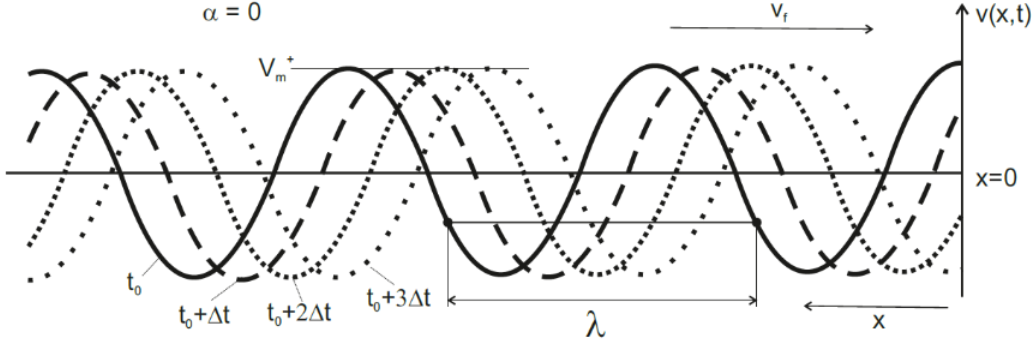
\includegraphics[width=\linewidth]{../assets/chap02_lossless_direct_wave.png}
					\caption[The direct voltage wave]{The direct voltage wave}
					\label{fig:chap02losslessdirectwave}
				\end{figure}
			
			\subsubsection{The direct current wave}
				The first term of the second equation in \ref{sec:volt+curr_lossless_line}, is called the \textbf{direct current wave}. This wave has the same properties as the direct voltage wave. 
			
			\subsubsection{The indirect waves}
				The second term of both equations are called the \textbf{indirect or reflected voltage and current wave}. They also have similar properties to the direct voltage wave, but they travel in the opposite direction. They are represented by the second term of each equation if section \ref{sec:volt+curr_lossless_line}.
				
			\subsubsection{The standing wave}
				The standing wave in a transmission line is the result of the superposition of a direct and indirect travelling wave with opposite directions of propagation.  Figure \ref{fig:chap02_standing_wave} is an example of these standing waves, each line depicts a voltage along the line at a different time instance.  The point at which the envelope of the lines reaches a maximum is called an \textbf{anti-node} and the minimum is called a \textbf{node}.
				
				\begin{figure}[h]
					\centering
					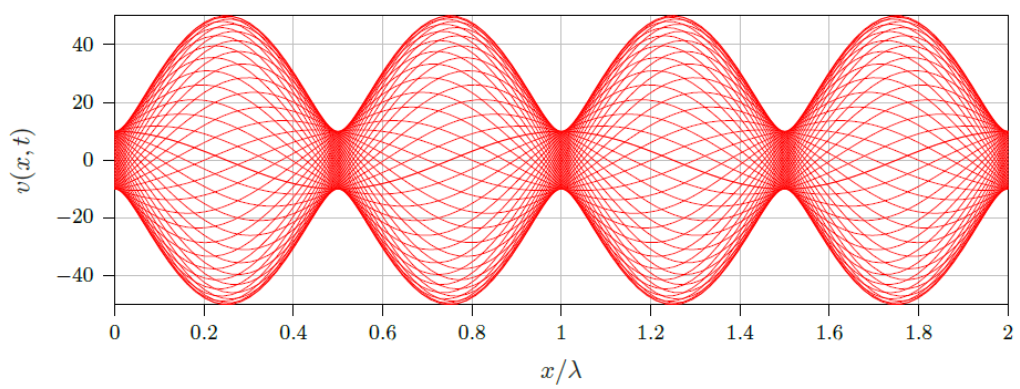
\includegraphics[width=\linewidth]{../assets/chap02_standing_wave.png}
					\caption{Example of a standing wave pattern on a transmission line}
					\label{fig:chap02_standing_wave}
				\end{figure}
		
		\subsection{The voltage reflection coefficient $\Gamma$}
			The \textbf{reflection coefficient} $\Gamma$ is defined as the ratio of the phasor of the reflected voltage wave to the phasor of the direct voltage wave. It can be defined at any point on the line and is thus a function of $x$.
			
			The modulus of $\Gamma$ expresses the \textbf{amplitude ratio} of the direct and indirect wave, while the phase of $\Gamma$ indicates the \textbf{phase difference} between the two. At places where the phase difference is an even multiple of $\pi$ we get constructive interference, and thus an anti-node in figure \ref{fig:chap02_standing_wave}, an odd multiple gives us destructive interference and thus we get a node. \\
			\\
			Finally, we have the following formulas for calculating $\Gamma$:
			\begin{equation}
				\Gamma(x=0) = \frac{Z_L-R_0}{Z_L+R_0} = \Gamma_L
			\end{equation}
			and
			\begin{equation}
				\Gamma(x)=\Gamma_Le^{-j2\beta x}
			\end{equation}
\end{document}
